\begin{frame}{Alternating Reset Depths in One Simulated Run}
\setlength{\abovedisplayskip}{4pt}
\setlength{\belowdisplayskip}{4pt}
\begin{columns}[T,onlytextwidth]
\begin{column}{0.54\textwidth}
\centering
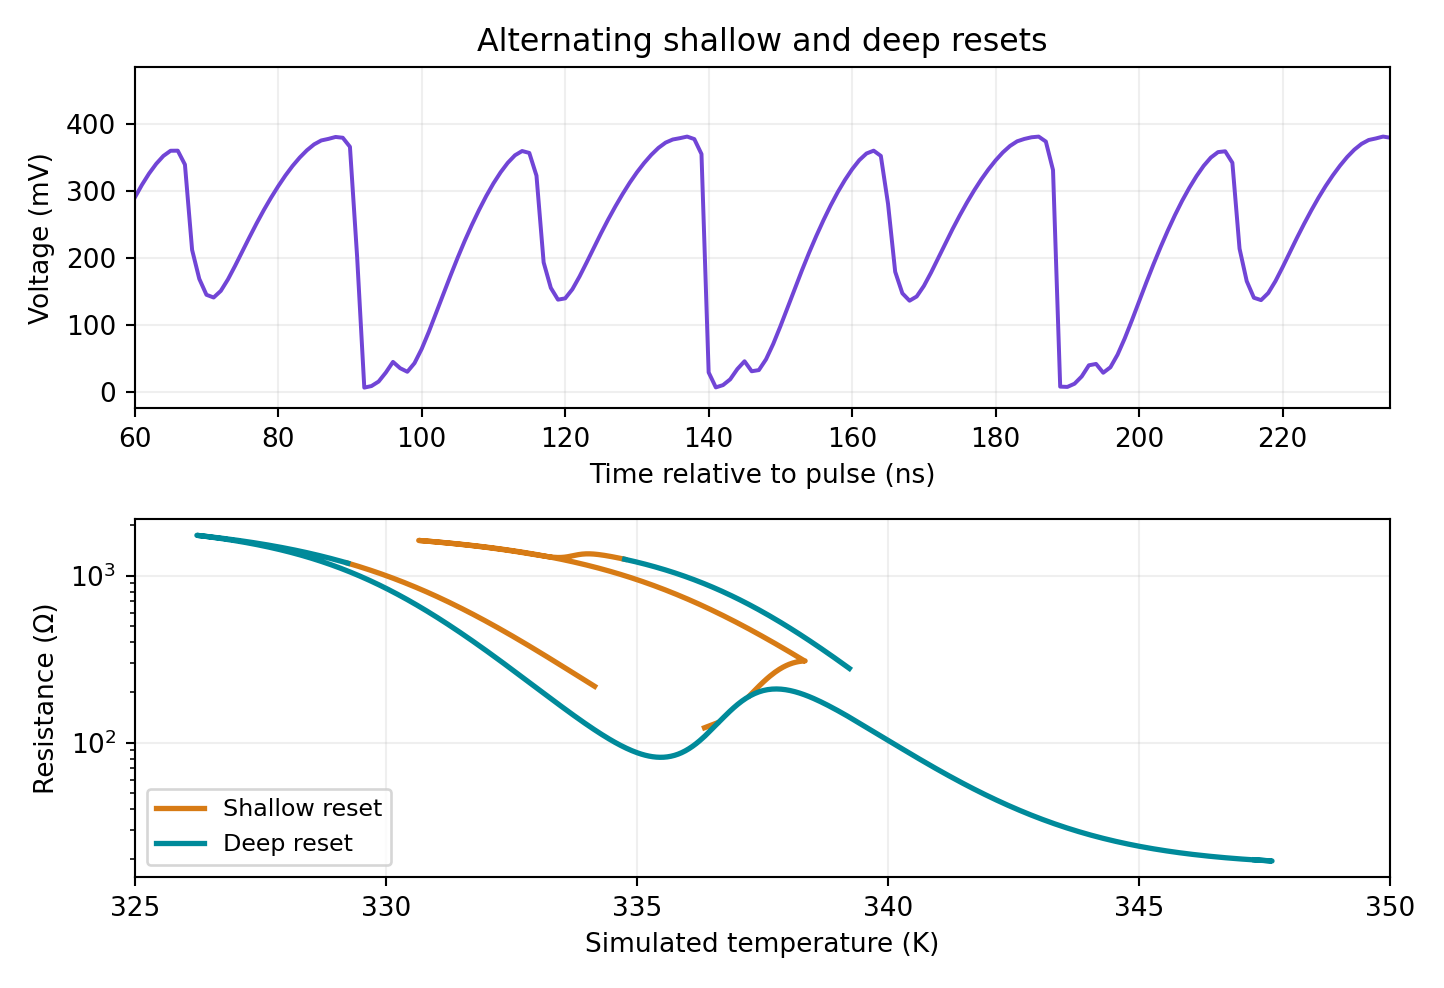
\includegraphics[width=\linewidth,height=.54\textheight,keepaspectratio]{alternating_resets_for_slide.png}
\par\vspace{0.04cm}\scriptsize
Source label 400 mV (about 303 \(\mu\)A).\\
Successive voltage swings: about 240 and 350 mV Vpp.
\par\vspace{0.12cm}
\localhtmlbutton{alternating-gifs}{Open the 44 current / voltage / R(T) GIFs}
\end{column}
\begin{column}{0.43\textwidth}
\small
\textbf{Two relevant time scales}
\[
\tau_{th}=\frac{C_{th}}{S_e}=11.91\ \mathrm{ns}
\]
\[
\tau_e(t)=C R(T,\mathcal H)
\simeq 0.13\text{--}12\ \mathrm{ns}
\]
\par\scriptsize
Along the displayed replay. Fully metallic limit:\quad
\(C R_m=0.125\ \mathrm{ns}\).
\par\vspace{0.15cm}\small
\textbf{Working explanation}
\par\vspace{0.04cm}\footnotesize
RC recharge competes with thermal recovery.
Hysteresis memory could alternate partial (about 338 K) and deep (about 348 K) resets.
\par\vspace{0.13cm}\scriptsize
\(C=6.835\) pF, \(C_{th}=0.04421\) pJ/K,\\
\(S_e=3.713\ \mu\)W/K, \(\gamma=0.15696\).
\end{column}
\end{columns}
\par\vspace{0.10cm}\footnotesize
\textbf{Numerical limit:} short-window alternation survives refinement.
Longer constant-current runs remain timestep-sensitive. Stable period doubling is unproven.
\slidesource{Historical diagnostic at 314.363 K, original specimen. Source 717797; audit 1072ef; GIFs 4b9e8c. The causal mechanism remains a hypothesis.}
\note{The thermal value is the passive cooling scale Cth/Se, not a third independent fitted constant or the full electrothermal relaxation eigenvalue. Electrical CR changes with the hysteretic resistance. The displayed original-timestep replay spans roughly 0.13 to 12 ns in 50--280 ns; CRm is 0.125 ns. Individual shallow cycles reach about 338 K with minimum R about 120 ohm, while deep cycles reach about 348 K and about 20 ohm. At high R, electrical recharge and thermal recovery are comparable. Deep low-R resets discharge much faster and create a different thermal and hysteresis reversal history. This is a plausible explanation for cycle-to-cycle memory, not a causal bifurcation proof. The 2 microsecond constant-current control becomes irregular at the finest tested step. C and gamma lie outside the historical constrained intervals. The button opens all 22 measured-current inputs at two timesteps with the same saved vector.}
\end{frame}
